\begin{frame}{Anexo 2}

\framesubtitle{Evaluaci�n - Matriz de Confusi�n}
\begin{center}
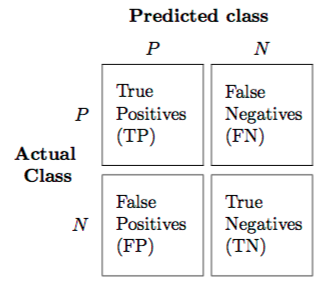
\includegraphics[width=0.6\textwidth]{anexo/graphics/confusion_matrix}
\par\end{center}

\end{frame}
%
\begin{frame}{Anexo 2}

\framesubtitle{Evaluaci�n - M�tricas de Evaluaci�n}

\setbeamercovered{transparent}
\begin{columns}

\column{0.3\textwidth}
\begin{itemize}[<+->]
\item Precisi�n 
\item Exhaustividad 
\item Exactitud 
\item Valor-F
\end{itemize}

\column{0.7\textwidth}
\begin{overprint}
\onslide<1> 

\[
Precisi\acute{o}n=\frac{TP}{TP+FP}
\]

\begin{center}
\emph{valor predictivo positivo}
\par\end{center}
\onslide<2> 

\[
Exhaustividad=\frac{TP}{TP+FN}
\]

\begin{center}
\emph{tasa positiva verdadera}
\par\end{center}
\onslide<3> 

\[
Exactitud=\frac{TP+TN}{TP+TN+FP+FN}
\]

\begin{center}
\emph{rendimiento general}
\par\end{center}
\onslide<4> 

\[
Valor-F=2\cdot\frac{Precisi\acute{o}n\cdot Exhaustividad}{Precisi\acute{o}n+Exhaustividad}
\]

\begin{center}
\emph{media arm�nica}
\par\end{center}

\end{overprint}
\end{columns}

\end{frame}
%
\begin{frame}{Anexo 2}

\framesubtitle{Evaluaci�n - Coeficiente de confiabilidad}
\begin{center}
\begin{tabular}{|c|c|c|}
\hline 
Valor & Nivel de acuerdo & \% de datos confiables\tabularnewline
\hline 
\hline 
0 - 0.20 & No & 0 - 4\%\tabularnewline
\hline 
0.21 - 0.39 & M�nimo & 4 - 15\%\tabularnewline
\hline 
0.40 - 0.59 & D�bil & 15 - 35\%\tabularnewline
\hline 
0.60 - 0.79 & Moderado & 35 - 63\%\tabularnewline
\hline 
0.80 - 0.90 & Fuerte & 64 - 81\%\tabularnewline
\hline 
>0.90 & Casi perfecto & 82 - 100\%\tabularnewline
\hline 
\end{tabular}
\par\end{center}

\end{frame}
%
\begin{frame}{Anexo 2}

\framesubtitle{Costo - Validaci�n cruzada}
\begin{center}
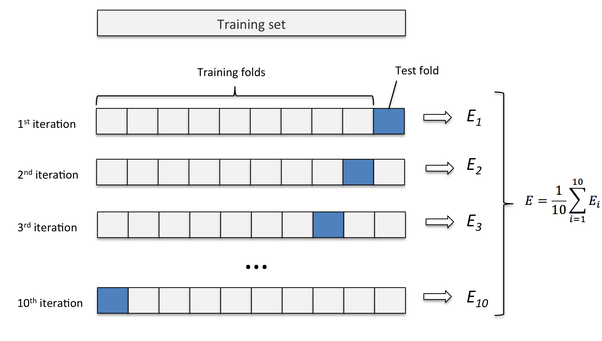
\includegraphics[width=1\textwidth]{anexo/graphics/ten_fold}
\par\end{center}

\end{frame}
%
\begin{frame}{Anexo 2}

\framesubtitle{Costo - M�tricas de Errores}

\setbeamercovered{transparent}
\begin{columns}

\column{0.5\textwidth}
\begin{itemize}[<+->]
\item Error absoluto
\item Ra�z de Error cuadr�tico medio
\item Error absoluto relativo
\item Ra�z de Error cuadr�tico relativo
\end{itemize}

\column{0.5\textwidth}
\begin{overprint}
\onslide<1> 

\[
E_{ma}=\frac{1}{n}\sum_{i\text{=1}}^{n}\bigl|y_{i}-f(x_{i})\bigr|
\]

\onslide<2> 

\[
E_{rms}=\sqrt{\frac{1}{n}\sum_{i\text{=1}}^{n}\left(y_{i}-f(x_{i})\right)^{2}}
\]

\onslide<3> 
\begin{center}
\[
E_{ra}=\sum_{i\text{=1}}^{n}\frac{\bigl|y_{i}-f(x_{i})\bigr|}{\bigl|y_{i}-\bar{y}\bigr|}
\]
con 
\[
\bar{y}=\frac{1}{n}\sum_{i=1}^{n}y_{i}
\]
\par\end{center}
\onslide<4> 
\begin{center}
\[
E_{rrs}=\sqrt{\sum_{i\text{=1}}^{n}\frac{\left(y_{i}-f(x_{i})\right)^{2}}{\left(y_{i}-\bar{y_{i}}\right)^{2}}}
\]
con 
\[
\bar{y}=\frac{1}{n}\sum_{i=1}^{n}y_{i}
\]
\par\end{center}
\end{overprint}
\end{columns}

\end{frame}

